\documentclass[12pt, oneside]{article}   	% use "amsart" instead of "article" for AMSLaTeX format

\usepackage{graphicx}
\graphicspath{ {\string} }
\usepackage{subcaption}

%%%%%%%%%%%%%%%%%%%%%%%%%%%%%%%%%%%%%%%%%%%%%%%%%%%%
% set up packages
%%%%%%%%%%%%%%%%%%%%%%%%%%%%%%%%%%%%%%%%%%%%%%%%%%%%
\usepackage{geometry}                
\usepackage{textcomp}                
\usepackage{amsmath}                
\usepackage{graphicx}                
\usepackage{amssymb}                
\usepackage{fancyhdr}                
\usepackage{subcaption}                
\usepackage{bm}                
\usepackage{lineno}

% package for comments
\usepackage{soul}     
\usepackage{setspace}

\usepackage{mathtools}
\usepackage{physics}

%%%%%%%%%%%%%%%%%%%%%%%%%%%%%%%%%%%%%%%%%%%%%%%%%%%%
% call packages
%%%%%%%%%%%%%%%%%%%%%%%%%%%%%%%%%%%%%%%%%%%%%%%%%%%%	
\geometry{letterpaper, marginparwidth=60pt} % sets up geometry              		
\linenumbers % adds line numbers 
\doublespacing % setspace
	
\usepackage[superscript,noadjust]{cite} % puts dash in citations to abbreviate
%\usepackage [autostyle, english = american]{csquotes} % sets US-style quotes
%\MakeOuterQuote{"} % sets quote style

\usepackage{hyperref}
\hypersetup{
    colorlinks=true,
    linkcolor=blue,
    filecolor=magenta,      
    urlcolor=cyan,
}

\usepackage{tabularx}

\usepackage{etoolbox}
\AtBeginEnvironment{quote}{\small}

\usepackage{float,color}
\usepackage{xcolor}
\definecolor{darkspringgreen}{rgb}{0.09, 0.45, 0.27}

\usepackage[section]{placeins}

\usepackage{tikz-qtree}
\usetikzlibrary{trees}

\usepackage{natbib}
%\bibliographystyle{abbrvnat}
\setcitestyle{authoryear,open={(},close={)}}

%%%%%%%%%%%%%%%%%%%%%%%%%%%%%%%%%%%%%%%%%%%%%%%%%%%%

%%%%%%%%%%%%%%%%%%%%%%%%%%%%%%%%%%%%%%%%%%%%%%%%%%%%
\pagestyle{plain}                                                      %%
%%%%%%%%%% EXAFT 1in MARGINS %%%%%%%                                   %%
\setlength{\textwidth}{6.5in}     %%                                   %%
\setlength{\oddsidemargin}{0in}   %% (It is recommended that you       %%
\setlength{\evensidemargin}{0in}  %%  not change these parameters,     %%
\setlength{\textheight}{8.5in}    %%  at the risk of having your       %%
\setlength{\topmargin}{0in}       %%  proposal dismissed on the basis  %%
\setlength{\headheight}{0in}      %%  of incorrect formatting!!!)      %%
\setlength{\headsep}{0in}         %%                                   %%
\setlength{\footskip}{.5in}       %%                                   %%
%%%%%%%%%%%%%%%%%%%%%%%%%%%%%%%%%%%%                                   %%		

%%%%%%%%%%%%%
% DEFINE CODE BLOCK
%%%%%%%%%%%%%
\usepackage{listings}

\definecolor{dkgreen}{rgb}{0,0.6,0}
\definecolor{gray}{rgb}{0.5,0.5,0.5}
\definecolor{mauve}{rgb}{0.58,0,0.82}

\lstset{frame=tb,
  language=R,
  aboveskip=3mm,
  belowskip=3mm,
  showstringspaces=false,
  columns=flexible,
  basicstyle={\small\ttfamily},
  numbers=none,
  numberstyle=\tiny\color{gray},
 % keywordstyle=\color{blue},
  commentstyle=\color{dkgreen},
  stringstyle=\color{mauve},
  breaklines=true,
  breakatwhitespace=true,
  tabsize=3,
  otherkeywords={0,1,2,3,4,5,6,7,8,9},
  deletekeywords={data,frame,length,as,character,dunif,ps},
}

%%%%%%%%%%%%%%%%%%%%%%%%%%%%%%%%%%%%%%%%%%%%%%%%%%%%
\usepackage{tikz}
\usetikzlibrary{arrows,automata}
\usetikzlibrary{positioning}

%%%%%%%%%%%%%%%%%%%%%%%%%%%%%%%%%%%%%%%%%%%%%%%%%%%%

%\usepackage{todonotes}

\begin{document} 
 
   	Last updated: \today

\section*{Resource allocation models}

The plant growth model developed by \cite{cohen1971} and later elaborated by \cite{King1982a} represents resources allocated to vegetative and reproductive pools. I summarize the model in equations \ref{eqn:de-resource} and \ref{eqn:constraints-resource} and state diagram \ref{fig:state-resource}. In the model, $x_1$ and $x_2$ are the weights of the vegetative and reproductive parts of the plant, respectively. Photosynthesis is assumed to be linearly related to the weight of the vegetative part of the plant. The control function $u(t)$ is the proportion of photosynthate that is allocated to the vegetative pool.

\cite{King1982a} propose that the long-term, optimal reproductive strategy will maximize the geometric mean of reproductive success. They propose that the function that should be optimized is the expectation of the log of fitness, $ J = (1/T) \int_{0}^{T} \mathrm{log}(x_2) \dd {t}$. They used the following system of equations:
%
\begin{align}
\dot{x_1} & = u(t) x_1 \nonumber \\
\dot{x_2} & = (1-u(t)) x_1 
\label{eqn:de-resource}
\end{align}

\noindent subject to
%
\begin{align}
0 \leq u&(t)  \leq 1 \nonumber \\
0  < x_1,&\ 0  \leq x_2 
\label{eqn:constraints-resource}
\end{align}

\begin{figure}[!h]
\centering
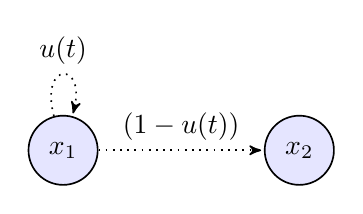
\begin{tikzpicture}[->,>=stealth',shorten >=1pt,auto,node distance=3cm,
                    semithick]
  \tikzstyle{every state}=[fill=blue!10,draw]    
   \node [state] (a) { $x_1$ };
    \node [state] (c) [right of=a] {$x_2$};
    \path[dotted, ->] (a) edge node {$(1-u(t))$} (c);
    \path[dotted] (a) edge [loop above] node {$u(t)$} (a);
\end{tikzpicture}
  \caption{State diagram describing the photosynthate allocation model.}
  \label{fig:state-resource}
\end{figure}

\hl{Describe some key results from this paper.}

\cite{King1982a} discuss how the model can be transformed to include a rate of growth ($r$) by substituting $t' = rt$. The differential equations are then
%
\begin{align}
\dot{x_1} & = u(t) r x_1 \nonumber \\
\dot{x_2} & = (1-u(t)) r x_1 
\label{eqn:transform-resource}
\end{align}

The growth rate constant $r$ in equation \ref{eqn:transform-resource} summarizes birth and death processes, $r = b - d$.

The resource allocation model can be shown to be a subset of models that represent development with meristems (compare Figure \ref{fig:state-resource} and \ref{fig:state-determinate-transform}). First, primary meristems divide into primary meristems and vegetative meristems. This is the process of vegetative growth. The second kind of division is when primary meristems divide into primary meristems and inflorescence meristems. So we can write the growth rate constant as the difference between meristem `birth' rate ($\beta_1$) and `death' rate ($\alpha$): $r = \beta_1 - \alpha$. In plants with a determinate inflorescence, all inflorescence meristems are converted to floral meristems. So if we only consider the vegetative and inflorescence meristem pools (Figure \ref{fig:state-determinate}), we obtain a model analogous to the resource allocation model. \hl{In the resource allocation model, flowering draws on vegetative biomass accumulated during vegetative growth but does not deplete vegetative biomass.}

\hl{UPDATE EVERYTHING BELOW THIS LINE}

\hl{A model in which $ r = 1 $ is one (for example) in which two primary meristems are produced and one is removed during each division (through death or quiescence). From a meristem perspective, this means accumulating meristems along an axis. From a resource perspective, this means accumulating a pool of photosynthetically active material. When $p(t)<1$, the interpretation would be that either some of those meristems begin to flower (and having more meristems means more flowering) or that resources are available to support reproduction.}

\begin{figure}[hbt!]
\centering
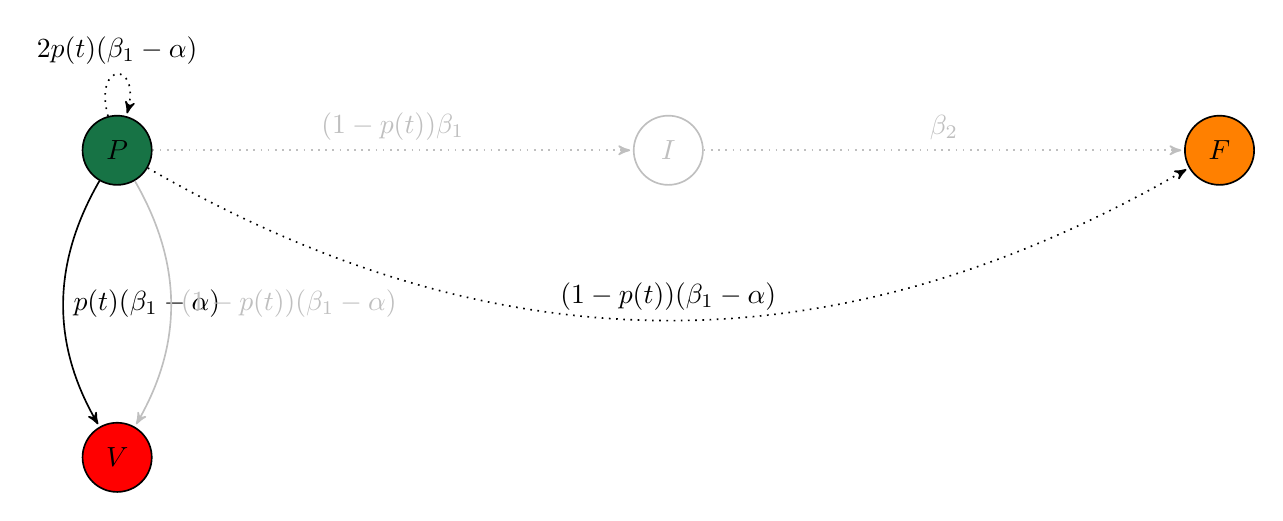
\begin{tikzpicture}[->,>=stealth',shorten >=1pt,auto,node distance=7cm,
                    semithick]
  \tikzstyle{every state}=[draw]    
   \node [state, fill=darkspringgreen] (a) { $P$ };
    \node [state, lightgray] (c) [right of=a] {$I$};
    \node [state, fill=orange] (d) [right of=c] {$F$};    
    \node [state, fill=red] (e) [below = 3cm of a] {$V$};    
    
    \path[dotted, ->,lightgray] (a) edge node {$(1-p(t)) \beta_1  $} (c);
    \path[dotted] (a) edge [loop above] node {$ 2 p(t)  (\beta_1 - \alpha) $} (a);
    %\path[dotted] (c) edge [loop above] node {$\beta_2$} (c);   
    \path[dotted, ->,lightgray] (c) edge node {$\beta_2$} (d);    
    \path[dotted] (a) edge[bend right] node {$( 1-p(t) ) (\beta_1 - \alpha) $} (d);
    \path (a) edge [bend right] node {$ p(t) (\beta_1 - \alpha) $} (e);
    \path[lightgray] (a) edge [bend left] node {$ ( 1-p(t) )(\beta_1 - \alpha)  $} (e);

\end{tikzpicture}
  \caption{State diagram describing the dynamics for plants with determinate inflorescences reduced to resource allocation model.}
  \label{fig:state-determinate-transform}
\end{figure}

Figure \ref{fig:state-determinate-transform} shows how the meristem allocation model contains the resource allocation model. By removing inflorescence meristems I limit the system to two types of divisions. In the first, primary meristems divide and produce more primary meristems (and leave behind a vegetative meristem). This division happens with probability $p(t)$. In the second, primary meristems divide and produce floral meristems. This happens with probability $1-p(t)$. 

The goal of this optimization problem is to maximize $F$. The variable in the model is $T$, the length of the season. The model is described by the following system of differential equations:
%
\begin{align}
\dot{P} & = 2 r p(t) P - r p(t) P \nonumber \\
\dot{V} & = r p(t) P \nonumber \\
\dot{F} & = r ( 1-p(t) ) P 
\label{eqn:de-determinate}
\end{align}

The differential equations describe the dynamics of three state variables: $P$, $V$, and $F$. I'm not sure where to go from here.

\textcolor{red}{SPE: To make meristem-based models into resource-allocation models, say that each division requires a certain amount of resources, so the rate at which they can happen is limited by the rate of photosynthesis. Instead of being parameters, $\beta_1$ and $\beta_2$ would be control variables, with the additional constraint that the total resource investment in meristem divisions can't exceed the rate of photosynthesis, something like}

\textcolor{red}{$c_1 \beta_1 p P + c_2 \beta_1 (1-p) P + c_3 \beta_2 I  \le \mathrm{constant}\times \mathrm{total\ leaf\ area} $}

\textcolor{red}{and maybe upper limits on the maximum possible division rate. Not sure how total leaf area would be determined in this model - proportional to total number of primary meristems? GS: My thought is to have a fourth pool that is not dynamic (it is just added to in the same way as F) but accumulates parent meristems after divisions. This pool of parent meristems can set the total leaf area. New question: are the betas now proportions or free controls?}


\clearpage
\bibliographystyle{/Users/gregor/Dropbox/bibliography/styleFiles/ecology} 
\bibliography{/Users/gregor/Dropbox/bibliography/optimal-control-lit}

\end{document}